\documentclass[../Main.tex]{subfiles}

\begin{document}

\subsection{Problems and obstacles}
One significant problem when attempting to use machine learning for tree/plant classification is the lack of existing datasets for training purposes. Especially for tree barks and for species typical for Easter Europe. The most of the existing datasets contain only a very small number of images as well as a limited number of classes. The reason for this is simple - researchers have to collect data manually by taking photos in order to start their work. 
There are also some large datasets, but majority of them are private or not publicly available. Fortunately, tremendous job done by authors of similar projects \cite{treebark2018} \cite{Robert2020BarkRe-Id} \cite{leafsnap_eccv2012} \cite{plantnet-db} \cite{leafsnap-db} enhance the possibilities to collect sufficient amount of data. 
For purpose of this project, different datasets are required - one with images of tree barks, and the second one - consisting of various plant images such as flowers, leaves or wide-photo.

\subsection{BarkNet 1.0}
    \subsubsection{Background}
    Authors of \textit{Tree Species Identification from Bark Images Using Convolutional Neural Networks} paper \cite{treebark2018} collected images from 23 different species of trees found in parks and forests. They were able to gather 23 000 cropped tree bark images in aggregate. 
    
    Photo was taken for each selected tree and than followed by 10-40 images of the bark at different locations and heights around this tree, depending on its circumference (using 4 different cellphone cameras). Images were captured at a distance between 20-60 cm away from the trunk. Forestry specialist was asked to identify every chosen tree.

    All images were taken so as to have the trunk parallel to the vertical axis of the image plane of the camera.
    Authors tried to ensure that the dataset would be as diversified as possible, so photos were taken under distinct weather condition and under various daylight.

    \subsubsection{Structure}
    Each photo in the database contains:
    \begin{itemize}
        \item unique number identifying the tree
        \item tree species
        \item DBH (diameter)
        \item camera used to take a photo
        \item date and time at which it was taken 
    \end{itemize}

    \begin{figure}[H]
        \centering
        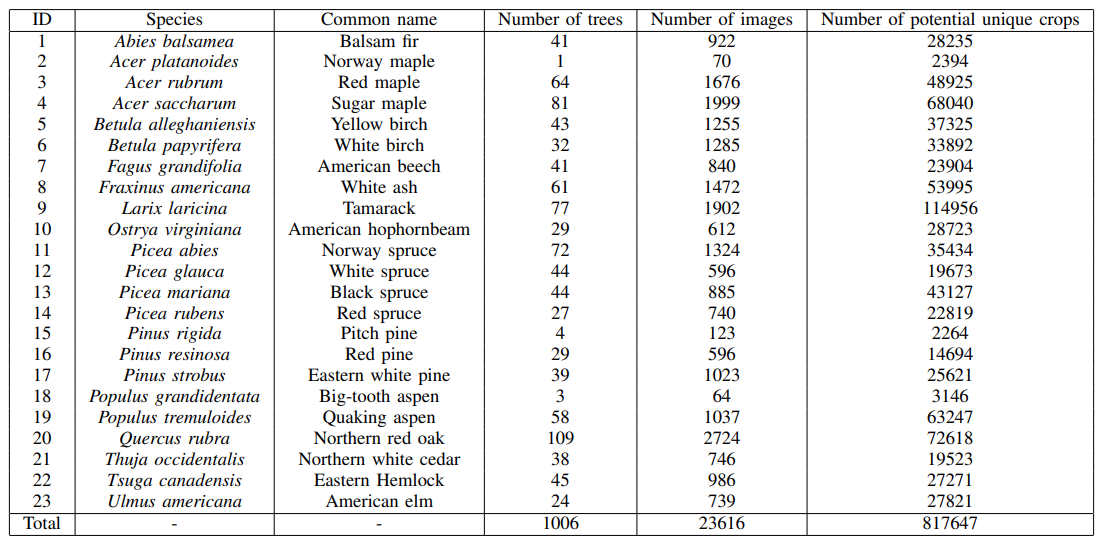
\includegraphics[width=0.9\textwidth]{Images/datasets/04_treebark_table.png}
        \caption{BarkNet 1.0 dataset composition \cite{treebark2018}}
        \label{fig:plantnet-voting}
    \end{figure}
    
    \subsubsection{Image examples}
    
    \begin{figure}[ht]
        \centering
        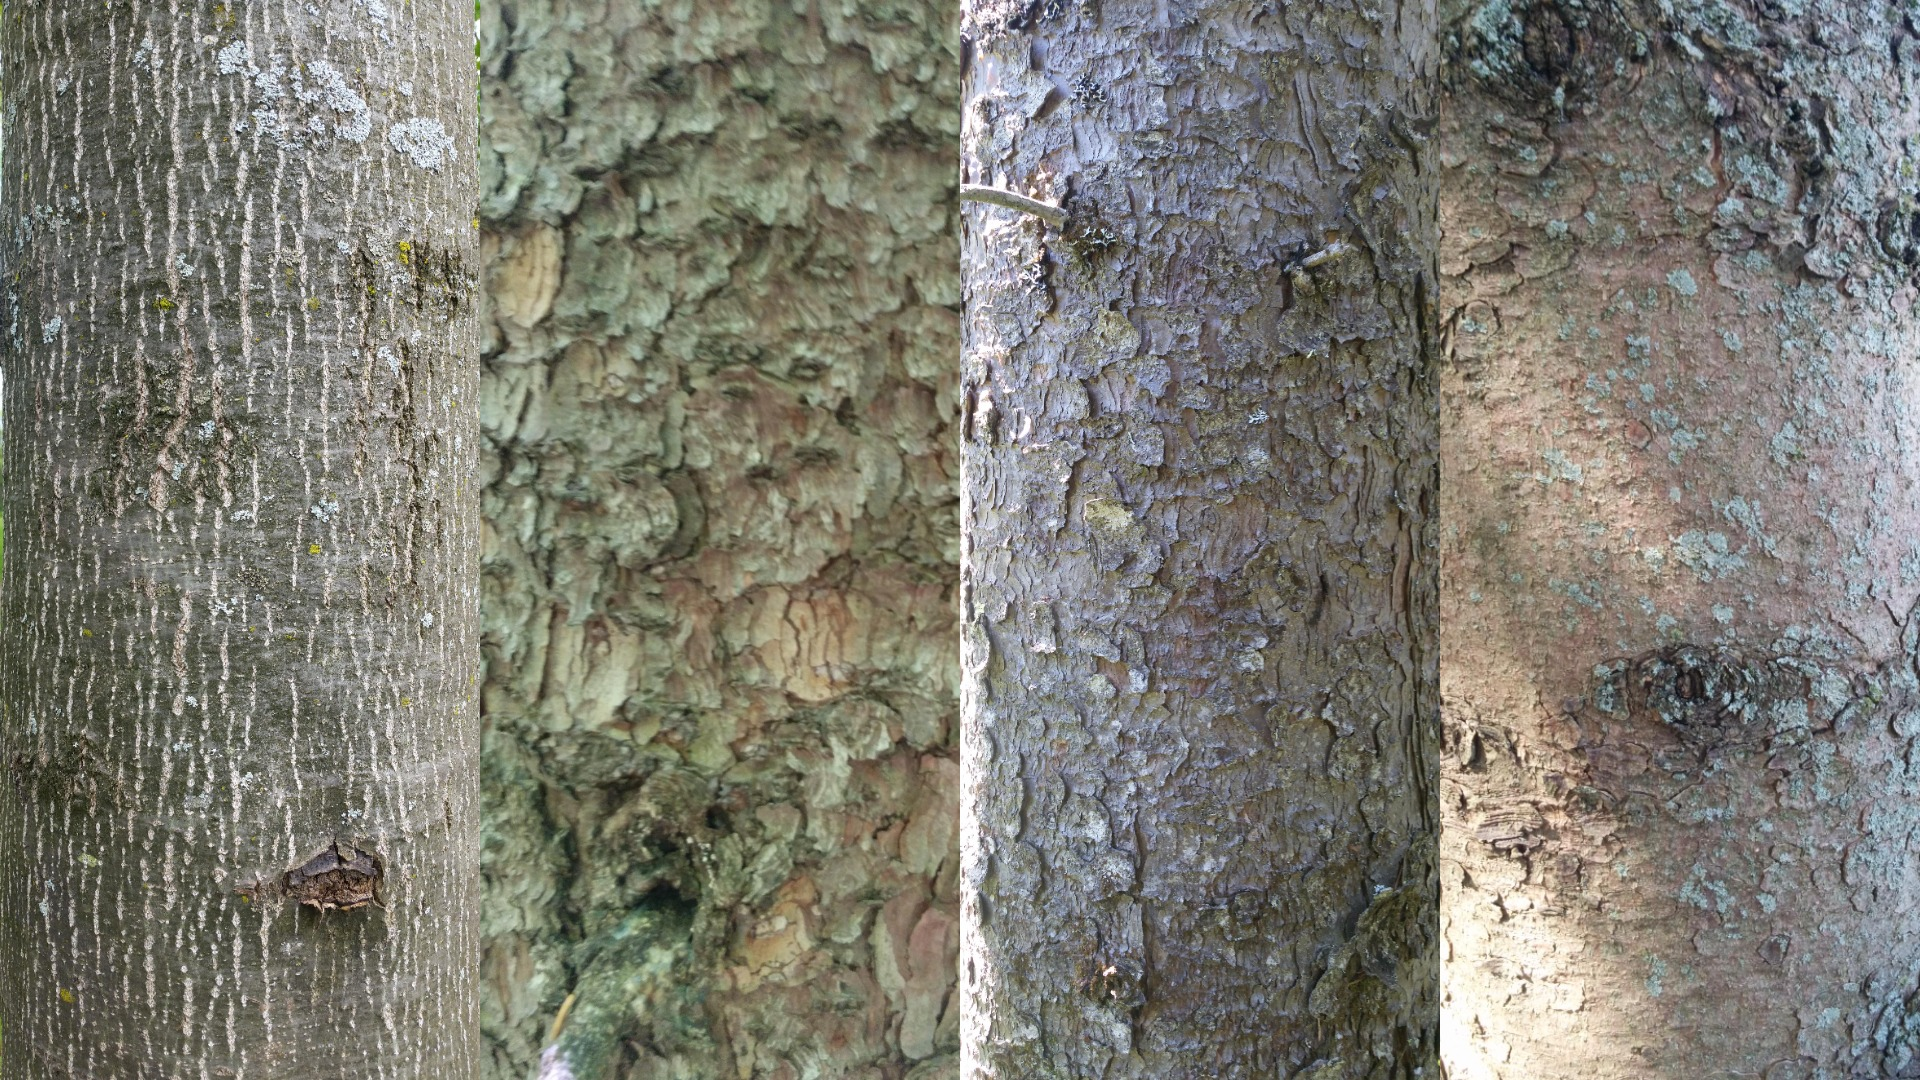
\includegraphics[width=0.9\textwidth]{Images/datasets/04_treebark_combined.jpg}
        \caption{4 cropped images from BarkNet 1.0 Dataset \cite{treebark2018}}
            \label{fig:04_treebark_combined}
    \end{figure}
    
    
\subsection{PlantNet}
    \subsubsection{Background}
    This dataset is a subsampling of the full dataset set used to train the models of the Pl@ntNet application (https://plantnet.org/). It comprises 1081 species of plants, representing a total of 306293 images \cite{plantnet-db}. It was created by randomly sampling the full Pl@ntNet dataset at the genus level. The data are composed of images collected through a citizen sciences initiative that was initiated in collaboration with Tela Botanica (social network of amateur and expert botanists). This makes data closer to the conditions of a real-world application: images of the same species are coming from distinct plants living in distinct areas; pictures are taken by different users that might not used the same protocol to acquire the images; pictures are taken at different periods in the year. 

    \subsubsection{Structure}
    Each image is associated with the following meta-data: \cite{clef}
    \begin{itemize}
        \item FileName
        \item MediaId
        \item View Content: Branch, Entire, Flower, Fruit, Leaf, LeafScan, Stem
        \item ClassId: the class number ID that must be used as ground-truth. It is a numerical taxonomical number used by Tela Botanica
        \item Genus: the name of the Genus, one level above the Species in the taxonomical hierarchy used by Tela Botanica
        \item Family: the name of the Family, two levels above the Species in the taxonomical hierarchy used by Tela Botanica
        \item Date: (if available) the date when the plant was observed,
        \item Vote: the (round up) average of the user ratings on image quality
        \item and other data, depending on part of dataset
    \end{itemize}

    Vote metadata is important annotation included for most of the pictures. These annotations are collectively produced by the Tela Botanica members through a collaborative web tool called pictoflora released in 2013.

    \subsubsection{Image examples and voting system}
    More the value is close to 5, more the organ is well photographed, typically a close-up photo where the organ covers a wide surface of the picture, sharp while the background is optically blurred thanks to a short deep-of-field, and thus with a clear and useful visual content for helping the plant identification. At the opposite, more the value is close to 1, less the picture is helpful for identifying the species for various reasons: the picture is globally blurred or the organ is out of focus, the organ is to small or/and the background is predominant with a sharp visual content like grass or leafage of other plants, the organ is too damaged like old fruit or dry leaves, some external object like a ruler, a pen or a coin for giving some information on size, etc.
    
    \begin{figure}[H]
        \centering
        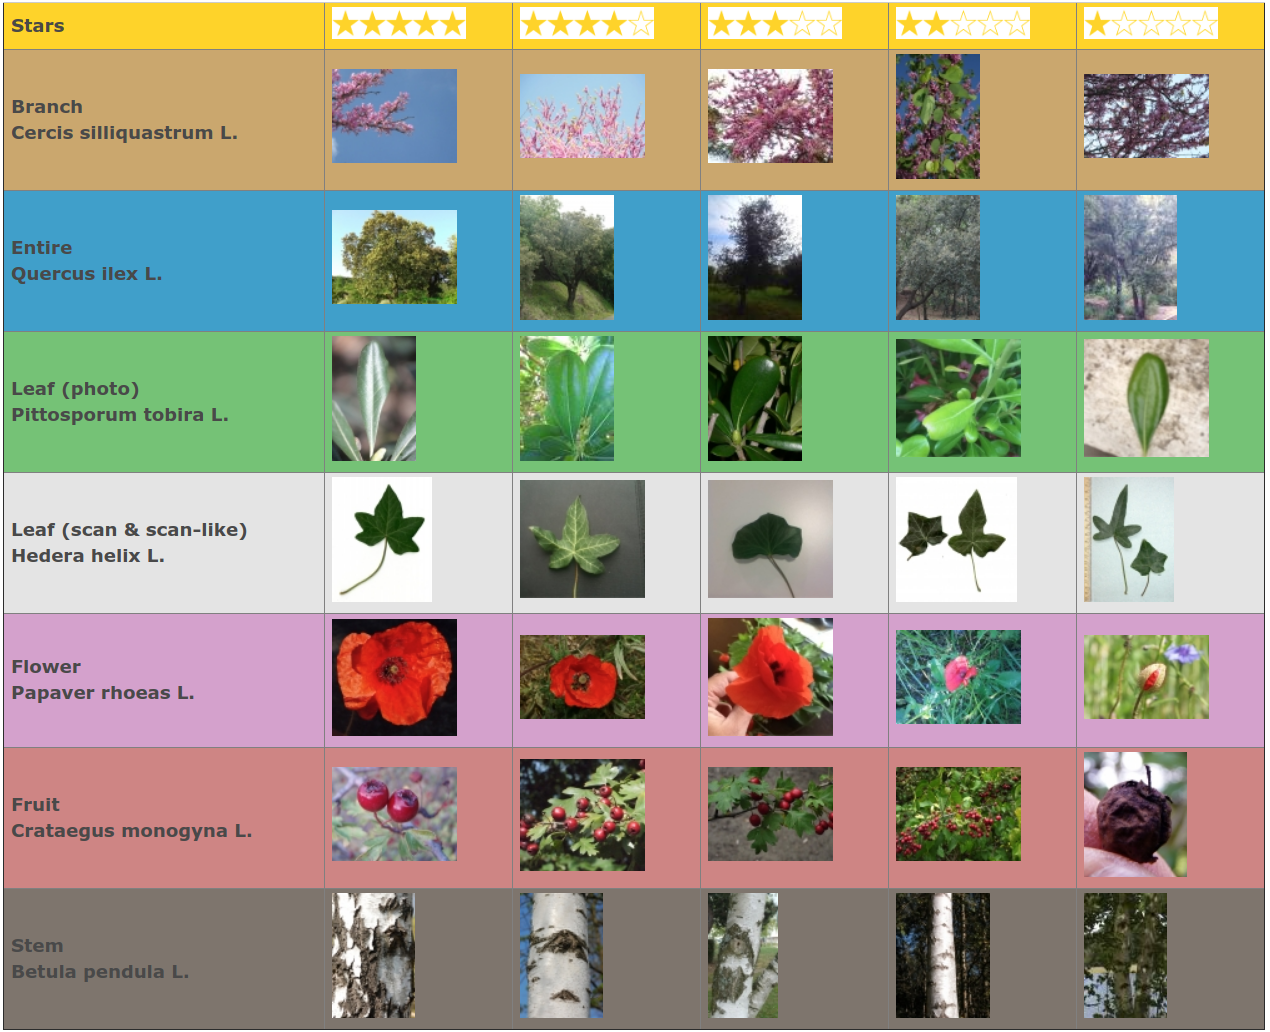
\includegraphics[width=0.9\textwidth]{Images/datasets/04_plantnet_voting.png}
        \caption{Images from PlantNet Dataset with wit votes (stars) assigned \cite{plantnet-db}}
        \label{fig:plantnet-voting}
    \end{figure}
    
\subsection{Leafsnap}

    \subsubsection{Background}
    The Leafsnap Database is a carefully collected database created by Columbia University, the University of Maryland, and the Smithsonian Institution. They were working on visual recognition software to help identify species from photographs and created Leafsnap as a series of electronic field guides being developed to demonstrate their new technologies. \cite{leafsnap_eccv2012} 
    
    The Original Leafsnap includes trees found in the Northeastern United States and Canada, and will soon grow to cover the trees of the entire continental United States. Leafsnap UK includes trees from across the United Kingdom with species information and imagery provided by the Natural History Museum in London. The part of dataset used for training and testing purposes of this project, currently covers all 185 tree species from the Northeastern United States. It was released on July 11, 2014 and has size of 977MB, so its pretty lightweight.
    
    \subsubsection{Structure}
    Leafsnap Dataset includes: \cite{leafsnap-db}
    \begin{itemize}
        \item 23147 Lab images, consisting of high-quality images taken of pressed leaves, from the Smithsonian collection. These images appear in controlled backlit and front-lit versions, with several samples per species.
        \item 7719 Field images, consisting of "typical" images taken by mobile devices (iPhones mostly) in outdoor environments. These images contain varying amounts of blur, noise, illumination patterns, shadows, etc.
    \end{itemize}
    
    The included leafsnap-dataset-images.txt file contains a listing of all the images, in tab-separated format (tsv). The first line is the header row, which describes each column:
    \begin{center}
        \begin{tabular}{ |c|c|c|c|c| } 
             \hline
             file\_id & image\_path & segmented\_path & species & source \\
             \hline
        \end{tabular}
    \end{center}
    
    Each line lists information about a single image. There are 5 fields, which are separated by tabs:
    \begin{enumerate}
        \item A unique numerical id for each image. These are not guaranteed to be consecutive or in order. They will not change over future versions of the dataset.
        \item The path of the original image.
        \item The path of the segmented version of the image. Note that where segmentation fails, the images might be completely black. In our running system, we have an automated check to discard such images from inclusion in the dataset for recognition.
        \item The scientific name of the species of the image. Note that these can have spaces and hyphens, and are in mixed case.
        \item The source of the image. This is either lab or field.
    \end{enumerate}
    
    \subsubsection{Image examples}
    This table shows example images and their segmentation for a few species (\ref{fig:03_leafsnap1}-\ref{fig:03_leafsnap1_4}):
    
    \begin{figure}[H]
        \minipage{0.5\textwidth}
            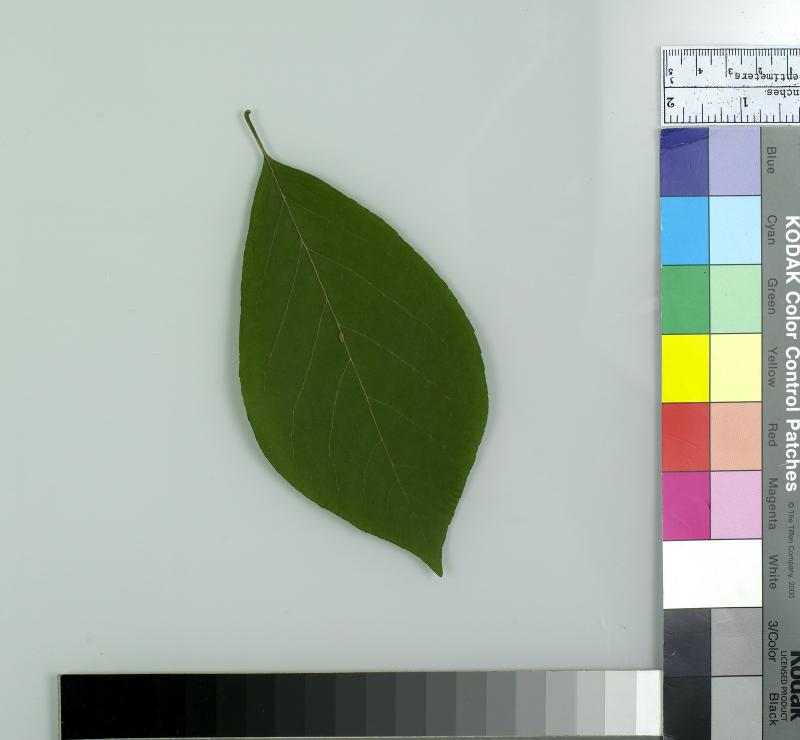
\includegraphics[width=\linewidth]{Images/datasets/03_leafsnap1.jpg}
            \caption{Example lab image}
            \label{fig:03_leafsnap1}
        \endminipage\hfill
        \minipage{0.5\textwidth}
            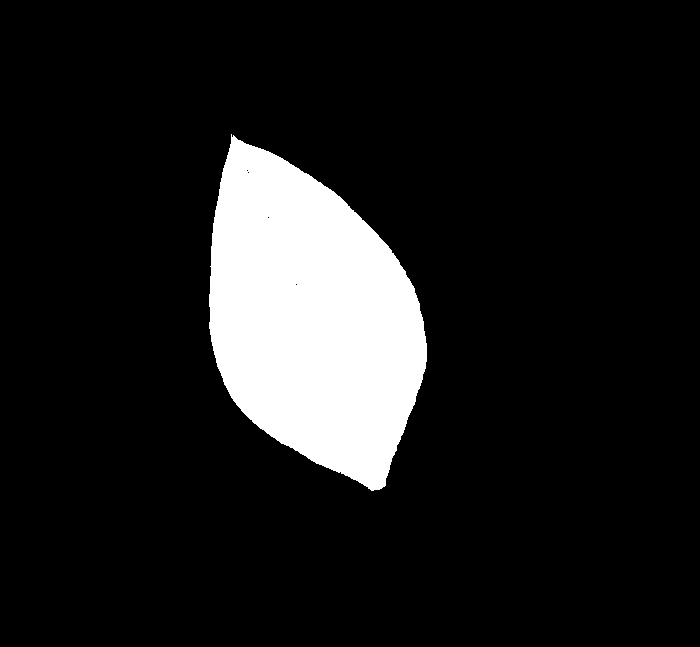
\includegraphics[width=\linewidth]{Images/datasets/03_leafsnap1_2.png}
            \caption{Example lab segmentation}
            \label{fig:03_leafsnap1_2}
        \endminipage\hfill
    \end{figure}
    \begin{figure}[H]
        \minipage{0.5\textwidth}
            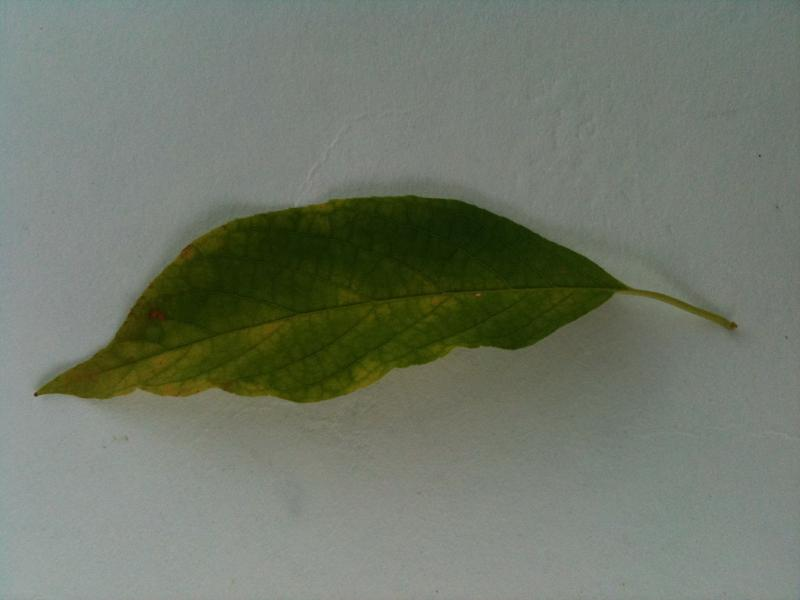
\includegraphics[width=\linewidth]{Images/datasets/03_leafsnap1_3.jpg}
            \caption{Example field image}
            \label{fig:03_leafsnap1}
        \endminipage\hfill
        \minipage{0.5\textwidth}
            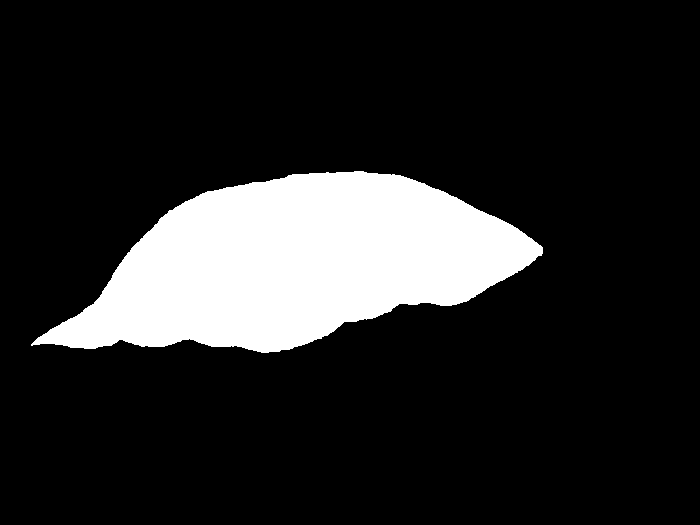
\includegraphics[width=\linewidth]{Images/datasets/03_leafsnap1_4.png}
            \caption{Example field segmentation}
            \label{fig:03_leafsnap1_2}
        \endminipage\hfill
    \end{figure}
    
    It is worth to mention that field images often come with poor quality, so human eye can hardly distinguishes between species. All photos were taken in laboratory - the leaves were placed on white background and artificially illuminated. Not always illimination was perfect, the examples of \textit{bad} images are presented on \ref{fig:03_leafsnap2}
    
    \begin{figure}[ht]
        \centering
        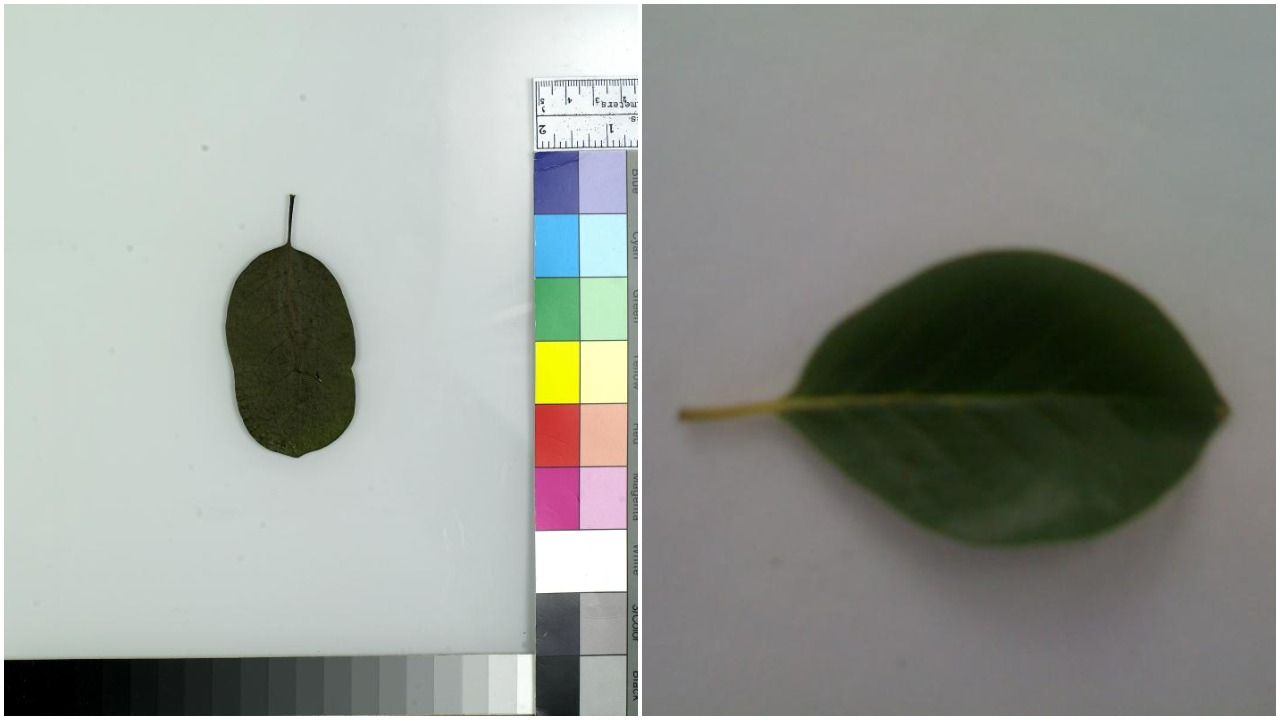
\includegraphics[width=0.8\textwidth]{Images/datasets/04_leafsnap2_combined.jpg}
        \caption{Poorly illuminated lab image and field image with bad quality \cite{leafsnap-db}}
            \label{fig:04_leafsnap2_combined}
    \end{figure}
    
\subsection{Other datasets}
    \subsubsection{Dendrodataset}
    There is a lack of rich databases consisting of only polish trees. The possibly useful one is Dendrodataset -  the dataset of 312 wood core images representing 14 European tree species, including both conifer and angiosperm (ring-porous and diffuse-porous) wood \cite{Fabijanska2021}.
    Unfortunately, it contains photographs presenting the internal part of tree trunk. Thus, the dataset is inadequate for purpose of this project. The user would have to take pictures of stubs or cut branches, what is obviously impossible.

    \begin{figure}[ht]
        \centering
        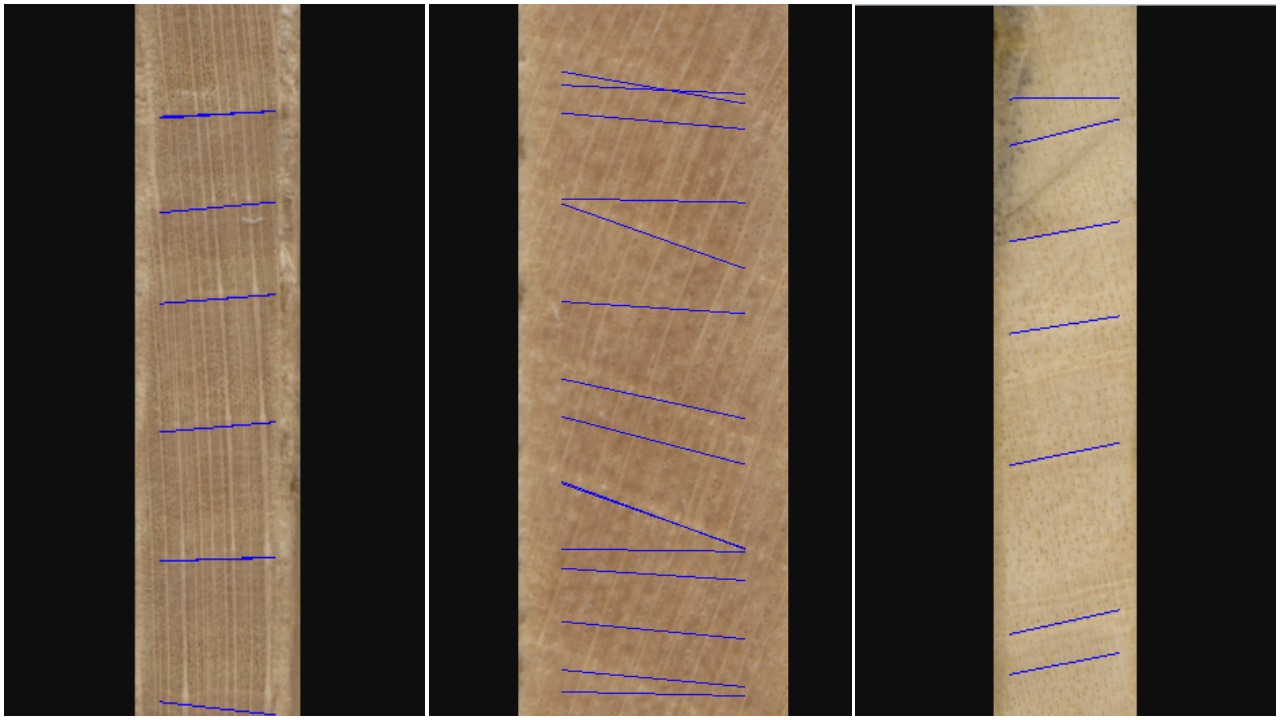
\includegraphics[width=0.7\textwidth]{Images/datasets/04_dendro_combined.jpg}
        \caption{Beech, tilia and betula\cite{Fabijanska2021}}
            \label{fig:04_dendro_combined}
    \end{figure}
    
    \subsubsection{Bark Datasets from Université Laval}
    The deficit of proper tree dataset forced authors of recent publications to collect data by themselves. Authors of \textit{Tree bark re-identification using a deep-learning feature descriptor} \cite{Robert2020BarkRe-Id} collected dataset with 200 uniquely-identified bark surface samples, for a total of 2,400 bark images. Using them, they produced a feature matching dataset enabling the training of deep learning feature descriptors.
    
    This dataset is publicly available and contains the unprocessed images we collected. Each of these images contains Red Pine or Elm bark, surrounded by our wooden frame. Images are organized by folder, with each folder representing a distinct bark surface. Also, each folder is identified by the tree species (EL or RP), the number of the tree, and the number of the surface of this tree used to take pictures.
    
    Another dataset created by this team is called Bark Aligned. It consists of images patches of 64x64 pixels. These patches are store as a numpy array with dimension (n, 12, 64, 64), where n is the number of keypoints found for a single bark surface. Each numpy file is identified with the same name as the folder in the Bark Id dataset to allow the correspondence between them. 
    
    Successful preprocessing and careful classification make this datasets really good source for future reaserchers.
    
    \begin{figure}[ht]
        \centering
        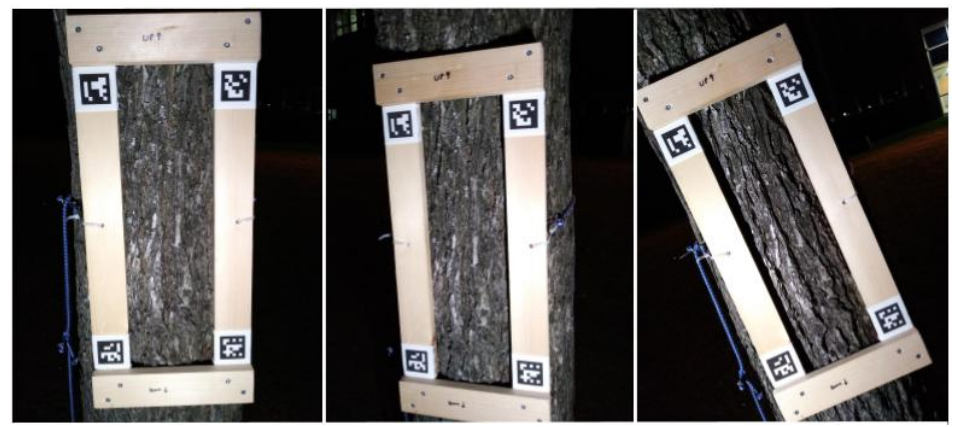
\includegraphics[width=0.7\textwidth]{Images/datasets/04_laval_shot.png}
        \caption{In each image, there are four fiduciary markers on a custom-made wooden frame, used for pixelwise registration.\cite{Robert2020BarkRe-Id}}
            \label{fig:04_laval_shot}
    \end{figure}

\newpage    

\biblio % Needed for referencing to working when compiling individual subfiles - Do not remove
\end{document}
